\documentclass{beamer}
\usepackage[francais]{babel}
\usetheme{metropolis}
\usepackage[utf8]{inputenc}
\usepackage[TS1,T1]{fontenc}
\usepackage{graphicx}
\usepackage{cprotect}
\usepackage{multirow}
\usepackage{eurosym}
\usepackage{supertabular}
\usepackage{amsmath}
\usepackage{hyperref}
\usepackage{kpfonts}
\usepackage{newunicodechar}
\newunicodechar{¬}{\TextOrMath{\textlnot}{\lnot}}
\newcommand{\textlongs}{{\fontencoding{TS1}\fontfamily{lmr}\selectfont\char115}}
\newboolean{FABR}
\setboolean{FABR}{true}

\cprotect\title{Exploiter des modèles de langue pour évaluer des sorties de logiciels d'OCR pour des documents français du XVII\ieme~siècle}
\author{Jean-Baptiste Tanguy}
\institute{CELLF, STIH, Sorbonne Université}

\begin{document}

	% Page de titre
	\begin{frame}
	\maketitle
	\end{frame}

	% Table des matières
	\begin{frame}
	\frametitle{Plan de la présentation}
	\begin{enumerate}
		\item Introduction
		\item \'{E}valuation non supervisée de sorties d'OCR
		\item Définition d'estimateurs de qualité d'OCR
		\item Expérience et résultats
		\item Perspectives
	\end{enumerate}
	\end{frame}

	% Introduction 1
	\begin{frame}\frametitle{Introduction}
		\begin{figure}[htbp] 
		\begin{center} 
		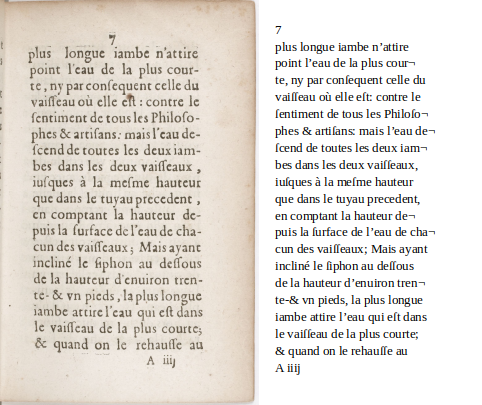
\includegraphics[scale=0.4]{pascal_15_img_transcription.png}
		\end{center} 
		\caption{Numérisation de la page 15 des \textit{Experiences Nouvelles touchant le vide…} de Pascal (1647) 
		présentée avec sa transcription diplomatique.} \label{pascal}
		\end{figure}
	\end{frame}

	% Introduction 2
	\begin{frame}\frametitle{Introduction}
		\begin{table}[h]
	    \begin{scriptsize}
	    \begin{tabular}{llll}
	    \multicolumn{1}{c}{\textbf{Lignes Kraken}} & \multicolumn{1}{l}{\textbf{CER}} & \multicolumn{1}{c}{\textbf{Lignes Tesseract}} & \multicolumn{1}{l}{\textbf{CER}} \\
	    plus longue iambe n'attire                 & 3,8 \%                         & plus Jongue iambe n'attire                    & 7,6 \%           \\
	    point lcau de la plus cour-                & 7,4 \%                         & point l'eau de la plus cour-                  & 3,7 \%           \\
	    te, ny par confequent celle du             & 3,4 \%                         & te, ny par confequent celle du                & 3,4 \%           \\
	    vaifeau oi elle ef : contre le             & 16,6 \%                        & vaiffeau où elle et : contre le               & 10 \%            \\
	    fentiment de tous les Philofo-             & 6,8 \%                         & fentiment de tous les Philofo-                & 6,8 \%           \\
	    phes artifans: maislcau de-                & 14,8 \%                        & phes \& artifans: mais l'eau de-              & 7,4 \%           \\
	    fcend de toutes lcs dcuxiam-               & 14,2 \%                        & fcend de toutes les deuxiam-                  & 7,1 \%           \\
	    bes dans les dcux vaiffeaux,               & 11,1 \%                        & bes dans les deux vaiffeaux ,                 & 7,4 \%           \\
	    iufques a la mefme hauteur                 & 11,5\%                         & iufques à la mefme hauteur                    & 7,6 \%            \\
	    que dans le tuyau preccdent,               & 3,7 \%                         & que dans le tuyau precedent ,                 & 0 \%             \\
	    en comptant la hautcur dec-                & 13,6 \%                        & en comptant la hauteur de-                    & 4,5\%           

	    \end{tabular}
	    \caption{Sorties d'OCR et \textit{CER} de Kraken et Tesseract pour le début de la page 15 des \textit{Experiences Nouvelles touchant le vide…} de Pascal (1647)} \label{ocr}
	    \end{scriptsize}
	    \end{table}
	\end{frame}


	% Introduction 3
	\begin{frame}\frametitle{Introduction}
		\'{E}valuation d'une sortie d'OCR : transcription diplomatique puis calcul du \textit{CER}, avec :
		$$CER = \frac{s + d + i}{C}$$
		
		Transcription diplimatique (au moins pour état de langue français du XVII\ieme):
		\begin{itemize}
			\item nécessite de l'expertise (philologie computationnelle) ;
			\item couteux temps ;
			\item nécessaire à toute évaluation.
		\end{itemize}

		\begin{center}
		Comment évaluer la qualité d'une sortie d'OCR \textbf{sans} vérité de terrain ? (\'{E}valuation non supervisée)
		\end{center}
	\end{frame}


	\section{\'{E}valuation non supervisée de sorties d'OCR}
		\begin{frame}\frametitle{\'{E}valuation non supervisée : plusieurs voies}
			\begin{itemize}
				\item Exploiter des ressources lexicales (la \textit{lexicalité} d'une sortie d'OCR) \cite{Springmann2016a} ;
				\item Exploiter les valeurs de confiance des logiciels d'OCR \cite{Springmann2016a} ;
				\item Exploiter les \textit{bounding boxes} \cite{Gupta2015a} ;
				\item (Reconnaissance de la parole) Exploiter les modèles de langue \cite{Chen1998a}.
			\end{itemize}
		\end{frame}

		\begin{frame}\frametitle{\'{E}valuation non supervisée : modèles de langue}
			Démarche :
			\begin{itemize}
				\item apprentissage de modèles de langue (grain caractère) sur des données textuelles françaises du XVII\ieme~siècle ;
				\item application des modèles d'OCR sur un corpus de documents numérisés du XVII\ieme~siècle ;
				\item calcul des \textit{CER} de ces sorties d'OCR (calculés avec les vérités de terrain) ;
				\item calcul d'estimateurs de qualité utilisant les modèles de langue.
			\end{itemize}

			Objectifs : 
			\begin{itemize}
				\item définir et calculer les estimatateurs de qualité d'OCR (exploitation des modèles de langue) ;
				\item étudier leurs corrélations avec les \textit{CER} (et les p-values).
			\end{itemize}
		\end{frame}

	\section{Définition des estimateurs de qualité d'OCR}
		\subsection{Exploiter les probabilités des modèles de langue}
		\begin{frame}\frametitle{Comment utiliser les modèles de langue ?}
			Les modèles de langue apprennent les probabilités que des caractères donnés suivent certaines séquences de caractères. 

			On peut donc :
			\begin{itemize}
				\item parcourir un texte par fenêtre glissante...
				\item ... récupérer la séquence de caractères contenue dans cette fenêtre ainsi que le caractère suivant...
				\item ... et récupérer la probabilité renvoyée par un modèle de langue pour que ce caractère suive cette séquence de caractères.
			\end{itemize}

			\begin{figure}[htbp] 
			\begin{center} 
			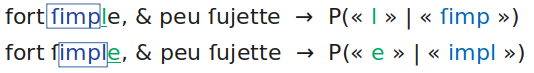
\includegraphics[scale=0.4]{Ex_proba_LM.png}
			\end{center} 
			\caption{Parcours d'un texte par fenêtre glissante (n=4) pour récupérer la probabilité d'un caractère sachant un historique.} 
			\end{figure}

		\end{frame}
		\begin{frame}\frametitle{Comment utiliser les probabilités des modèles de langue ?}	
			Hypothèse : ces probabilités peuvent être de bons indices pour estimer la qualité d'une sortie d'OCR 
			\begin{itemize}
				\item Océrisation douteuse $\Rightarrow$ suite de caractères qui n'est pas du texte $\Rightarrow$ faibles probabilités
				\item Océrisation de qualité $\Rightarrow$ suite de caractères formant du texte $\Rightarrow$ fortes probabilités
			\end{itemize}
		\end{frame}

		\subsection{Agréger les probabilités des modèles de langue}
		\begin{frame}\frametitle{Comment agréger les probabilités ?}
			\begin{footnotesize}
			La somme $S$, le produit $Pr$, la perplexité $Pp$ et le log-perplexité $log(PP)$ sont calculés pour chaque ligne puis moyennés sur la page

			$$S = \sum_{i=n+1}^{C-n}P_{LM}(c_{i} | h_{n,i})$$
			$$Pr = \prod_{i=n+1}^{C-n}P_{LM}(c_{i} | h_{n,i})$$
			$$PP = \frac{1}{(\prod_{i=n+1}^{C-n}P_{LM}(c_{i} | h_{n,i}))^{\frac{1}{C-n}}}$$
			
			$$log(PP)$$
			Avec $P_{LM}$ la probabilité renvoyée par un modèle de langue $LM$, $n$ 
	        la taille de la fenêtre glissante, $C$ le nombre total de caractères de la sortie d'OCR, $c_{i}$ 
	        le $i$\ieme~caractère de la sortie d'OCR et $h_{n,i}$ l'historique des $n$ caractères
	        \end{footnotesize}
		\end{frame}

	\section{Expérience et résultats}
		\subsection{Les corpus}
		\begin{frame}\frametitle{Les corpus}
		\cite{Gabay2019a} a rassemblé et transcrit plusieurs \oe{}uvres françaises du XVII\ieme~siècle 
		\begin{scriptsize}
		\begin{table}[h]		    
		    \begin{tabular}{|l|c|c|c|}
		    \multicolumn{4}{c}{i) Corpus pour l'apprentissage des modèles de langue}\\\hline
		    \textbf{Identifiant}&\textbf{Nb lignes}&\textbf{Nb mots}&\textbf{Nb caractères}\\\hline
		    Bossuet-1683&27&770&4~128\\ \hline
		    Chapelain-1656&28&753&4~735\\ \hline
		    Ellain-1606&22&618&3~168\\ \hline
		    Gournay-1622&31&825&4~284\\ \hline
		    \multicolumn{4}{c}{ii) Corpus pour l'océrisation et son évaluation}\\\hline
		    \textbf{Identifiant}&\textbf{Nb lignes}&\textbf{Nb mots}&\textbf{Nb caractères}\\\hline
		    Papin-1682&23&548&2~230\\ \hline
		    Pascal-1647&39&776&3~568\\ \hline
		    Sales-1641&25&618&3~915\\ \hline
		    Viau-1623&33&852&4~055\\\hline
		    \end{tabular}
		    \caption{Description des sous-corpus dédiés à i) l'apprentissage des modèles de langue et ii) l'océrisation
		    et l'évaluation de la qualité des sorties d'OCR.} \label{tab:souscorpus}
		\end{table} 
		\end{scriptsize}
		\end{frame}

		\subsection{Les technologies utilisées}
		\begin{frame}\frametitle{Les technologies utilisées}
		Pour l'OCR :
		\begin{itemize}
			\item \cite{Kiessling2019a} : Kraken, modèle pour l'anglais contemporain et modèle pour le français du XVII\ieme~siècle
			\item \cite{Smith2007a} : Tesseract, modèle pour l'anglais contemporain
		\end{itemize}

		Pour les modèles de langue :
		\begin{itemize}
			\item modèles de langue à probabilités conditionnelles
			\item modèles de langue appris par des réseaux de neurones (LSTM et biLSTM) (\textit{keras} de Python)
		\end{itemize}

		\end{frame}

		\subsection{Résultats}
		\begin{frame}\frametitle{Résultats}
		\begin{table}

		\begin{center}
	    \begin{tiny}
	    {\setlength{\tabcolsep}{0.1cm}
	    \begin{tabular}{l||cc|cc|cc|cc}  

	    \multirow{2}{*}{\textbf{}} & \multicolumn{2}{c}{\textbf{S}}         & \multicolumn{2}{c}{\textbf{Pr}}        & \multicolumn{2}{c}{\textbf{PP}}        & \multicolumn{2}{c}{\textbf{log(PP)}}   \\ 
	    & \textbf{corrélation} & \textbf{p-value} & \textbf{corrélation} & \textbf{p-value} & \textbf{corrélation} & \textbf{p-value} & \textbf{corrélation} & \textbf{p-value} \\ %\hline
	    \textbf{n=2}  & -0,004 & 0,968 & 0,158  & \textcolor{blue}{\textbf{0,086}}          & 0,113  & 0,221          & 0,006  & 0,952          \\ %\hline
	    \textbf{n=3}  & -0,130 & 0,156 & 0,009  & 0,920          & -0,003 & 0,976          & 0,056  & 0,540          \\ %\hline
	    \textbf{n=4}  & -0,124 & 0,178 & -0,005 & 0,960          & 0,016  & 0,866          & 0,060  & 0,518          \\ %\hline
	    \textbf{n=5}  & -0,158 & \textcolor{blue}{\textbf{0,084}} & -0,070 & 0,449          & 0,134  & 0,143          & 0,158  & \textcolor{blue}{\textbf{0,085}}          \\ %\hline
	    \textbf{n=6}  & -0,138 & 0,133 & -0,054 & 0,556          & 0,180  & \textcolor{blue}{\textbf{0,049}} & 0,188  & \textcolor{blue}{\textbf{0,040}} \\ %\hline
	    \textbf{n=7}  & -0,100 & 0,278 & -0,027 & 0,773          & 0,093  & 0,313          & 0,084  & 0,359          \\ %\hline
	    \textbf{n=8}  & -0,055 & 0,547 & -0,008 & 0,930          & -0,006 & 0,949          & -0,008 & 0,928          \\ %\hline
	    \textbf{n=9}  & -0,054 & 0,554 & -0,083 & 0,366          & 0,096  & 0,299          & 0,095  & 0,300          \\ %\hline
	    \textbf{n=10} & -0,024 & 0,796 & -0,212 & \textcolor{blue}{\textbf{0,020}} & 0,228  & \textcolor{blue}{\textbf{0,012}} & 0,187  & \textcolor{blue}{\textbf{0,041}} \\ %\hline
	    \end{tabular}}\label{tab:res_corr}
	    \end{tiny}
	    \end{center}  
	    \caption{Corrélations et \textit{p-values} calculées entre les métriques d'estimation et le \textit{CER}. OCR : Tesseract (anglais contemporain). ML : probabilités conditionnelles.}
	    \end{table}

	    La table ci-dessus est celle qui contient le plus de valeurs significatives (l'ensemble des résultats est présenté dans l'article). 

		\end{frame}

		\begin{frame}\frametitle{Résultats}

			\textbf{Très peu de corrélations significatives} entre les estimateurs et les \textit{CER} ($p\-values \gg 0.1$), et ce pour :
			\begin{itemize}
				\item les deux logiciels d'OCR ;
				\item les trois modèles d'OCR ;
				\item les quatre estimateurs ;
				\item tous les modèles de langue (proba conditionnelles, LISTM et biLSTM pour $n \in \llbracket 2~;~ 10 \rrbracket$).
			\end{itemize}
		\end{frame}

		\subsection{Explication}
		\begin{frame}\frametitle{Pourquoi ? \'{E}valuation des modèles de langue.}
		La perplexité peut être calculée pour évaluer les modèles de langue (sur une référence).
		\begin{scriptsize}
		
		\begin{table}[h]
	    \begin{center}
	    \begin{tabular}{|l|c|c|c|}
	    \hline
	                  & \textbf{ML probabilités conditionnelles} & \multicolumn{1}{r|}{\textbf{ML LSTM}} & \textbf{ML biLSTM} \\ \hline
	    \textbf{n=2}  & 90                                       & 14721                                 & 257646757092       \\ \hline
	    \textbf{n=3}  & 126                                      & 1010690                               & 235913940342       \\ \hline
	    \textbf{n=4}  & 426                                      & 318251055                             & 221055920422       \\ \hline
	    \textbf{n=5}  & 1091                                     & 723946838                             & 211044617070       \\ \hline
	    \textbf{n=6}  & 1978                                     & 690749546                             & 204520506752       \\ \hline
	    \textbf{n=7}  & 2801                                     & 669397958                             & 200184237186       \\ \hline
	    \textbf{n=8}  & 3510                                     & 655634987                             & 1161841181775      \\ \hline
	    \textbf{n=9}  & 3940                                     & 647905538                             & 13807745026062     \\ \hline
	    \textbf{n=10} & 4205                                     & 643364471                             & 14481238375005     \\ \hline
	    \end{tabular}\caption{Moyennes des perplexités des modèles de langue sur les transcriptions n'ayant pas servis à leur apprentissage.}\label{tab:perplex}
	    \end{center}
	    \end{table}
	    \end{scriptsize}
		\end{frame}

		\begin{frame}\frametitle{Pourquoi ? \'{E}valuation des modèles de langue.}
		\begin{itemize}
			\item Une perplexité faible suggère que le modèle de langue est de qualité (on prend généralement comme seuil d'acceptabilité 400)
			\item Le tableau précédent montre des valeurs \textbf{aberrantes}
			\item Sauf pour les modèles de langue à probabilités conditionnelles pour $n \in \llbracket 2~;~ 4 \rrbracket$
		\end{itemize}
		\end{frame}

\begin{frame}\frametitle{Perspectives}

\begin{itemize}
	\item Mauvaise qualité des modèles de langue $\Rightarrow$ impossibilité d'évaluer les estimateurs de qualité d'OCR
	\item Reconduire l'expérience avec plus de données pour apprendre les modèles de langue pour répondre aux questions suivantes :
	\begin{itemize}
		\item Les modèles de langue sont-ils finalement non adaptés à l'estimation de qualité d'OCR ?
		\item Sont-ce les estimateurs ?  
		\item Le corpus présente-t-il des spécificités telles que les modèles de ne peuvent être de bons indicateurs ?
	\end{itemize}
\end{itemize}
\end{frame}

%\begin{frame}\frametitle{Annexe : construction actuelle des réseaux LSTM et biLSTM}
%\begin{figure}[htbp] 
%\begin{center} 
%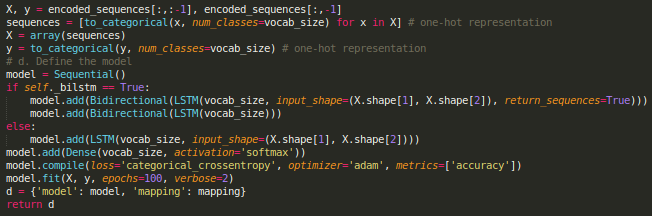
\includegraphics[scale=0.5]{reseau.png}
%\end{center} 
%\caption{Capture d'écran du code construisant les réseaux LSTM et biLSTM.}
%\end{figure}
%\end{frame}

\bibliographystyle{jeptaln2020}
\bibliography{historical_documents_OCR.bib}
 
\end{document}

